\section{Chapter 7: Inertial Confinement}

\subsection{What are typical orders of magnitude for terms in the triple product for magnetic and inertial confinement? What does this mean for steady-state operation?}
\solutionblock{See Figure \ref{fig:4_inertial_vs_magnetic}: \\
Magnetic Confinement: 
\[n \approx 10^{20} \text{ particles / m$^3$ },\quad T \text{ in range } 10 - 20 \text{ keV} \approx 100-200 \text{ million K}, \quad \tau_E \approx 10^{0.5} \text{ s}\]
Inertial Confinement: 
\[n > 10^{30} \text{ particles / m$^3$ },\quad T \text{ in range } 10 - 20 \text{ keV} \approx 100-200 \text{ million K}, \quad \tau_E \approx 10^{-9} \text{ s}\]
A typical value would be $nT\tau_E \approx 10^{21} \text{ m$^{-3}$ keV s}$.\\

Practically this means for the inertial confinement the energy gained by one pulse must be enough to heat the next fuel pellet. }

\subsection{Draw and explain an inertial fusion reaction by direct and indirect drive. How is it related to the hydrogen bomb?}
\begin{multisolutionblock}
    
    In the direct drive the laser beams are directly focused on the fuel pellet. In the indirect drive the laser beams are focused on a hohlraum which then heats the fuel pellet:\\
    \begin{figure}[H]
        \centering
        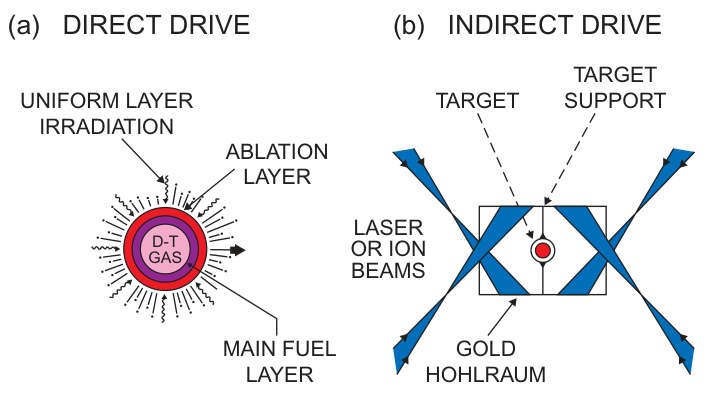
\includegraphics[width=0.65\textwidth]{chapters/fig/7_direct_indirect_drive.png}
        \caption{Comparison of the principles of direct and indirect drive. Uniform irradiation is
        produced by many laser beams in the direct-drive case and by the production of X-rays at the wall
        of the hohlraum in the indirect case. The targets are similar in size in the two cases, but the direct
        drive has been shown enlarged to illustrate the typical structure.}
        \label{fig:7_direct_indirect_drive}
    \end{figure}
    The hydrogen bomb uses a fission bomb to create the conditions for fusion. Both the bomb and inertial confinement creates the conditions for fusion by compressing the fuel pellet. While the bomb uses a fission bomb to compress the fuel pellet, inertial confinement uses (mainly) lasers to heat the outer layers which then compress the fuel pellet.
\end{multisolutionblock}


\subsection{How does a laser work? Discuss efficiency and future possibilities for technical break-even.}
\begin{multisolutionblock}
    A laser is a device that emits light through a process of optical amplification based on the stimulated emission of electromagnetic radiation. The term "laser" originated as an acronym for "light amplification by stimulated emission of radiation".\\
    \begin{figure}[H]
        \centering
        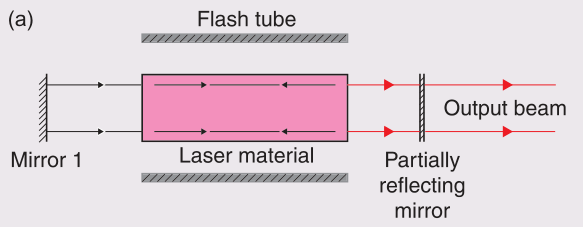
\includegraphics[width=0.65\textwidth]{chapters/fig/7_laser_schematics.png}
        \caption{Schematic diagram of a typical laser.}
        \label{fig:7_laser}
    \end{figure}
    In principle a laser pumps energy into a medium (gas, liquid or solid) which raises the electrons to a higher energy level. These electrons then fall back to a lower energy level if they are stimulated by a photon of the same energy as the energy drop between the two levels. This will cause the electron to emit a photon of the same energy as the stimulating photon. This process is called stimulated emission. These photons are then reflected back and forth between two mirrors stimulating more emissions on their way. One of the mirrors is partially transparent and lets some of the photons out. \\

    \begin{figure}[H]
        \centering
        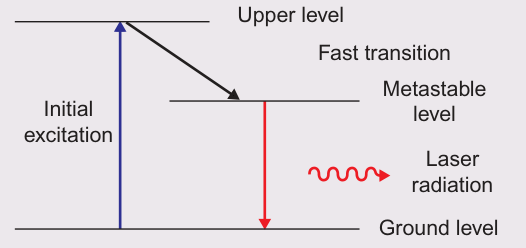
\includegraphics[width=0.65\textwidth]{chapters/fig/7_laser_principle.png}
        \caption{Principle of stimulated emission.}
        \label{fig:7_laser_principle}
    \end{figure}


\end{multisolutionblock}
